\section{Durchführung}
\label{sec:Durchführung}

\subsection{Apparatekonstante}
\label{subsec:app}
Für das Experiment wird ein Viskosimeter, wie in \autoref{Abb:viskosimeter} verwendet.



\begin{wrapfigure}{r}{5.5cm}
    \centering
    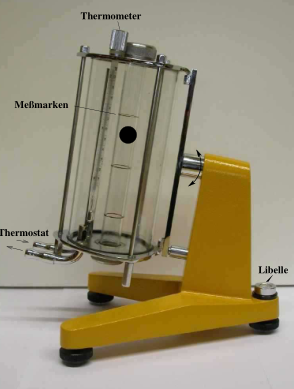
\includegraphics[width=5.5cm]{Dateien/Viskosimeter.png}
    \caption{Im Experiment verwendetes Viskosimeter \cite{anleitung107}.}
    \label{Abb:viskosimeter}
\end{wrapfigure}

Als erstes wird für die Bestimmung des Volumens der beiden Glaskugeln, mit denen das Experiment durchgeführt wird,
das Gewicht und der Radius, beziehungsweise der Durchmesser bestimmt. Im Experiment wird eine große und eine kleinere Kugel verwendet.

An der Seite, auf der der erste Strich näher am Ende der Röhre ist, wird ein Stopfen ohne Loch eingelassen und verschraubt.
An der Libelle wird das Viskosimeter gerade eingestellt.
Das Viskosimeter wird nun langsam mit destilliertem Wasser gefüllt, sodass keine Luftblasen in der Versuchsröhre %????
übrig bleiben. Falls doch welche im Viskosimeter sind, werden sie mit einem dafür vorgesehen Glasstab entfernt. Die kleinere Kugel
wird nun langsam in das Viskosimeter eingelassen.
Ein zweiter Stopfen mt einem kleinen Loch, sodass überschüssiges Wasser abfließen kann, wird in das zweite Ende eingelassen, danach mit einer
Gummischeibe versiegelt und anschließend zugeschraubt.

Es wird nun die Fallzeit der kleinen Kugel zwischen den äußersten Strichen gemessen. Dabei ist darauf zu achten, dass die Kugel,
wenn sie den ersten Messstrich erreicht, bereits eine konstante Geschwindigkeit hat. Dies ist üblicherweise beim ersten Strich der Fall.
Das Viskosimeter lässt sich um $\SI{180}{\degree}$ drehen und es werden die Fallzeiten der Kugel für beide Richtungen gemessen. Dabei
sollten die Heizschläuche nicht so sehr verfangen, dass sie sich lösen.
Es werden 10 Durchläufe bei Raumtemperatur des Wassers gemessen.

Mit der großen Kugel werden ebenfalls 5 Durchläufe bei Raumtemperatur durchgeführt.

\subsection{Temperaturäbhangigkeit von destilliertem Wasser}
\label{subsec:tempAbh}

Nun soll die Temperaturäbhangigkeit von destilliertem Wasser gemessen werden. Dafür werden jeweils zweimal die Fallzeiten der großen Kugel bei
unterschiedlichen Temperaturen von bis bis zu $\SI{50}{\celsius}$ gemessen. 
Das Wasserbad des Viskosimeters, welches um die Teströhre angebracht ist, wird auf eine Temperatur eingestellt und das Wasserbad wird erhitzt.
Es muss ein wenig gewartet werden, sodass das Wasser in der Teströhre auch dieselbe Temperatur von dem Wasserbad angemnommen hat.
Wurden zwei Durchläufe bei einer Temperatur durchgeführt, so kann eine höhere Temperatur eingestellt werden.